\section{Analysis of Solutions: Interpolation}
Similar to the discussion in Analysis of Solutions: Linear Systems, we have found different ways a student might implement one part of the method, in particular in the case of interpolation, we are referring to the lines of code that calculate what value does a point of the mesh (without the interpolation points) have as a y-coordinate. The portion of the code can be summarised as: 

Note that different algorithms might have a different calculation but for simplicity purposes we are generalizing the section of the code


\begin{algorithm}[H]
\SetAlgoLined
\For{$j \gets 1$ \KwTo $n-2$} {
$k[x_j <= u] \gets j$
}
$s \gets u - x_k$\\
$v \gets y_k + s * \Delta_k$

\caption{Extract from Interpolation's algorithm}
\end{algorithm}

The different ways we could think of implementing this portion of the code are:
\begin{enumerate}
    \item List Comprehension: Python offers a compact form for adding items to a list, in particular list comprehension, for a general reader a list comprehension is based on mathematical notation that is $\left\{ 3n\ |\ \forall n\in 0...25\right\}$ can be written in python as \lstinline|[3*n for n in range(0,26)]|, generally speaking list comprehension are faster than classical loops\cite{PythonSpeedPerformanceTips}, however a better approach would be using functional maps which are cognitively more difficult to understand thereby not the purpose of this project.

    \item Using NumPy's \textit{fancy} Indexing: Similar to Matlab, NumPy offers a way to broadcast a list, that is we can access the items of a list using another list, even though it is cognitively more complicated than list comprehensions, it is a syntax that is widely used in the numerical methods realm and might be a fair competitor over list comprehensions.
    
\end{enumerate}
\subsection{Results}
To correctly test the implementations we will fix 6 interpolation pairs, and then run 100 iterations for different mesh with random values (to also check the ability to sort the mesh points), then after those 100 iterations are over we will calculate the mean, the results are the following:
\begin{figure}[H]
    \centering
    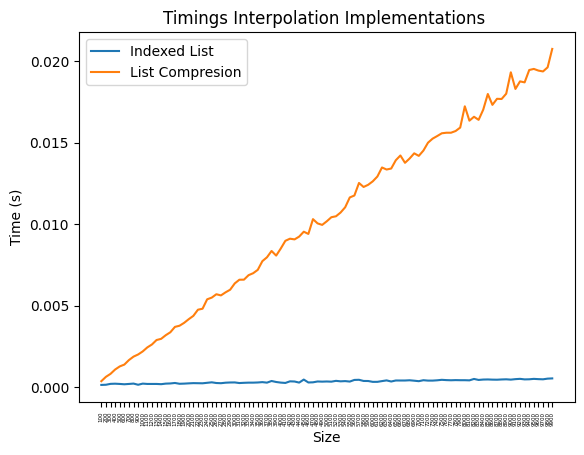
\includegraphics[scale=0.9]{Include/Images/Thesis/Analysis of Solutions/Interpolation/Interpolation Timings.png}
    \caption{Interpolation Timings}
    \label{fig:Interpolation Timings}
\end{figure}

As we can visually observer, the use of List Comprehesions is by far the worst of the two, and should be discarded for this particular case. We can also see by how much does the \textit{fancy} indexing improve the overall speed, that is why applying linear regression on the data, we have:
\begin{enumerate}
    \item \textbf{Linear Regression Indexed List}: \\
        y = 3.4812e-08x + 0.0002 \\
        Slope: 3.48119e-08
    \item \textbf{Linear Regression List Compresion}: \\
        y = 2.0237e-06x + 0.0003 \\
        Slope: 2.02374e-06
\end{enumerate}

Overall, not only does the choice of \textit{fancy} indexing is by far the fastest (around 2 order of magnitude) but it also provides students a syntax that will be used during their learning of numerical methods, though it must be noted, the use of for-loops might be ideal for didactic purposes to teach students what could be behind the notation of this \textit{fancy} indexing.